% How and why the system is structured that way

\chapter{Methodology}
\label{chap:method}

\section{Research Approach}
This thesis follows a design and implementation-oriented methodology aimed at developing and evaluating a privacy-preserving extension for Android applications using Custom Tabs (CTs) and Trusted Web Activities (TWA).
The main research goal is to prevent HyTrack's cross-app tracking attack \cite{USENIX:Wessels:2025} by eliminating the fundamental weaknesses \autoref{sec:hytrack-weaknesses} that enable such tracking while confirming to the design goals \autoref{sec:hytrack-goals} outlined by Wessels et al. without sacrificing usability or compatibility -- unlike Browser State Partitioning or Forced User Interaction \autoref{sec:hytrack-mitigations}.

We fill this gap by wrapping Cookies into fine-grained capability tokens -- created by the browser according to a policy defined by the app's developer --, the browser decides which cookies are stored in the shared cookie jar and which are stored in the app-specific storage, depending on a flag analogous to CHIPS' ~\cite{googlechips} \texttt{Partitioned} attribute.
This ensures that there is no cross-app tracking possible for untrusted third-party libraries, as each app stores its own tracking cookie.
As the shared cookie storage still exists for domains declared as first-party or trusted by the app developer, legitimate uses of the shared browser state (e.g. SSO) are preserved (Goal~3).
Because the system operates purely at the app–browser interface and does not alter the browser's rendering engine, it preserves compatibility with all existing web platform features (Goal~1).
Seamless integration of web content is also maintained, as there is no need for user interaction or changes to the UI (Goal~2).
Thus, in contrast to prior discussed mitigation strategies, this approach provides developers with a practical and enforceable way to render cross-app tracking infeasible.

% TODO: Write about our interpretation of capabilities here? -- how they enhance security/privacy explicity

To achieve this, a prototype framework named Byetrack was designed, implemented, and evaluated on Android.
The framework consists of three main components: a custom installer for policy extraction, a helper library for application integration, and modifications to the Mozilla Fenix browser and its underlying GeckoView engine to enforce cookie isolation via capability tokens.

% -----------------------Explain Methodology Flow Diagram Here ---------------------------
\section{Lifecycle and Flow}
\begin{figure}[h!]
  \centering
  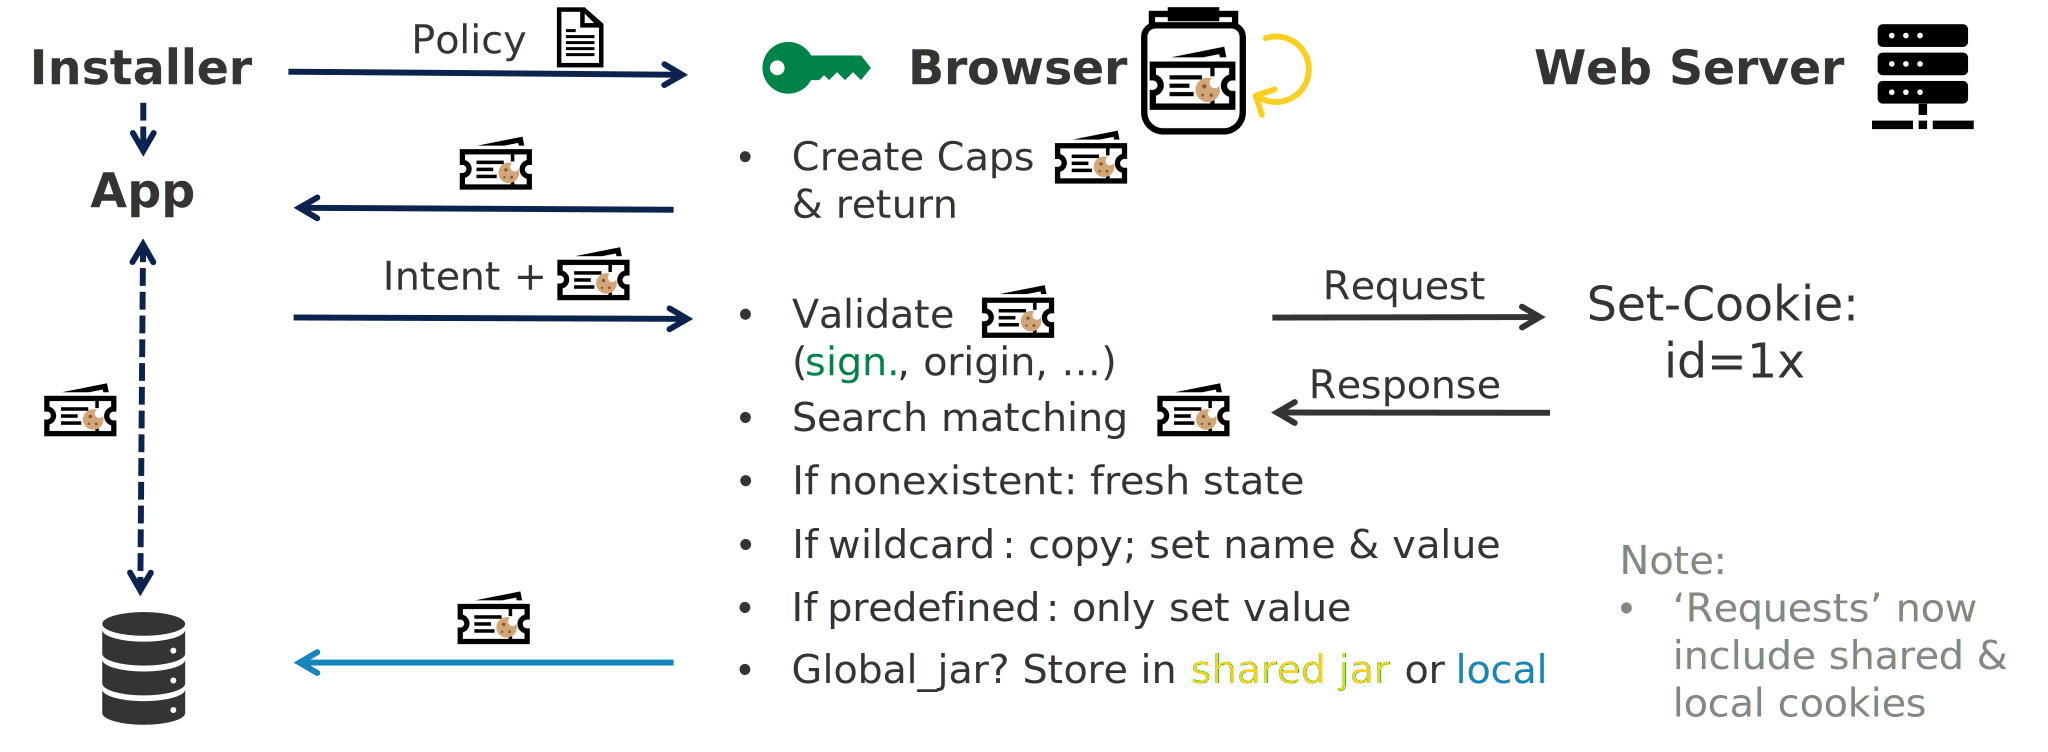
\includegraphics[width=0.9\textwidth]{ByeTrack_Flow.pdf}
  \caption{High-level overview of the Byetrack flow between installer, app, browser, and web servers.}
  \label{fig:byetrack_overview}
\end{figure}

\subsection{Developer Policy}
Developers define a JSON policy that specifies which domains may share browser state and, optionally, which cookies are expected from each domain.
This allows granular control beyond simple trusted/untrusted domain distinctions -- for example, isolating third-party cookies while permitting integration with a developer's own authentication domain or SSO provider.
If no policy is provided, the browser falls back to ambient mode, where all cookies are stored in the shared jar for backwards compatibility.

\subsection{Capability Initialization}
During app installation, the installer extracts and transmits the policy to the browser.
The browser validates and sanitizes the policy to ensure minimal privilege, removing conflicting or ambiguous entries.  

From the sanitized policy, the browser generates capability tokens as follows:
\begin{itemize}
  \item For predefined cookie entries, the browser creates corresponding predefined capability tokens.
  \item For domain-level entries, the browser issues wildcard capabilities, marking them as global or private based on the policy.
  \item If no policy is provided, a single ambient capability is issued, reverting to the default shared-cookie behavior.
\end{itemize}

Each token is signed and encrypted before being sent to the app, which stores wildcard and final tokens in private storage for later use.  
When the app is updated, the installer retransmits the policy so that the browser can reissue capabilities consistent with the new app version.

\subsection{App–Browser Interaction}
When an app opens a URL through a Custom Tab (CT) or Trusted Web Activity (TWA), the stored wildcard and (initially empty) final tokens are attached to the intent that launches the browser.
Upon receipt, the browser decrypts and validates each token by checking its signature, package name, version number, and target domain.
Invalid tokens are discarded.

The browser then uses the valid capabilities to:
\begin{enumerate}[label=\arabic*.]
  \item Determine how to store cookies received from the web server.
  \item Construct cookie headers for outgoing requests.
\end{enumerate}

\paragraph{Cookie Reception.}  
For every received cookie, the browser applies the following logic (in order of priority):
\begin{enumerate}[label=\arabic*.]
  \item If the token is ambient, the cookie is stored in the global jar (default behavior).
  \item If a private predefined capability matches the cookie name, the cookie value is filled in and returned to the app for local storage.
  \item If a private wildcard capability exists, the cookie is filled in accordingly and returned to the app.
  \item If a global predefined capability matches, the cookie is stored in the shared jar.
  \item If a global wildcard capability exists, any cookie from the corresponding domain is stored in the shared jar.
  \item If no capability matches, the cookie is discarded.
\end{enumerate}

\paragraph{Cookie Transmission.}  
When constructing requests, the browser merges cookies derived from the app's valid final tokens with those from its global jar, ensuring that each request accurately reflects both app-specific and shared state according to the developer policy.

% ---------------------------------------------------------------------------

\subsection{Utility Interfaces}
To improve transparency and developer control, the browser exposes limited utility functions that allow the app to:
\begin{enumerate}[label=\arabic*)]
  \item Retrieve the names of cookies encapsulated in final capabilities.
  \item Read their corresponding values.
  \item Write or update cookie values.  
\end{enumerate}
Access to these utilities is strictly controlled through capability rights: read operations require read rights, and modifications require write rights.

\section{Design Advantages}
Beyond preventing cross-app tracking, Byetrack offers several key benefits:
\begin{enumerate}[label=B\arabic*)]
  \item \textbf{Fine-Grained Control:} Developers can precisely specify which cookies are shared or isolated.
  \item \textbf{Stateless Browser Design:} The browser remains stateless with respect to app-specific data, as apps retain and transmit their own tokens.
  \item \textbf{No Web Server Changes:} Web servers operate unmodified—the browser transparently enforces the capability model.
  \item \textbf{Backwards Compatibility:} Apps without a policy fall back to the standard shared cookie behavior, ensuring compatibility with existing systems.
\end{enumerate}

\section{Alternative Design Considerations}
An alternative architecture would delegate capability generation to the installer rather than the browser.  
This would simplify the browser's responsibilities to enforcement only, reducing its complexity and eliminating installer–browser communication for each app.  
However, it would require shared cryptographic secrets between the installer and browser, thereby enlarging the trusted computing base and attack surface.  
For these reasons, the proof-of-concept implementation designates the browser as the sole trusted component for capability generation and enforcement.
